\documentclass[11pt,a4paper]{article}
\usepackage[a4paper,top=2.5cm,bottom=2.5cm,left=2.6cm,right=2.6cm]{geometry}
\usepackage[T1]{fontenc}
\usepackage[utf8]{inputenc}
\usepackage{mathptmx}
\usepackage{microtype}
\usepackage{amsmath,amssymb}
\usepackage{booktabs,array,multirow}
\usepackage{graphicx}
\usepackage{needspace}
\usepackage{url}\urlstyle{tt}
\usepackage{caption}
\usepackage{enumitem}
\usepackage{titlesec}
\usepackage{fancyhdr}
\usepackage[colorlinks=true,linkcolor=black,urlcolor=black,citecolor=black]{hyperref}

\graphicspath{{figures/}}
\setlength{\parindent}{1.4em}\setlength{\parskip}{0pt}
\renewcommand{\arraystretch}{1.12}
\setlength{\tabcolsep}{4.2pt}
\setlist{itemsep=1pt,topsep=2pt,parsep=0pt,leftmargin=1.5em}
\captionsetup{font=small,labelfont=bf,labelsep=space,justification=justified,singlelinecheck=false,skip=4pt}
\captionsetup[figure]{name=Fig.}
\captionsetup[table]{position=above}
\setlength{\textfloatsep}{14pt plus 2pt minus 4pt}
\setlength{\floatsep}{12pt plus 2pt minus 4pt}

\renewcommand{\thesection}{\Roman{section}}
\renewcommand{\thesubsection}{\thesection.\Alph{subsection}}
\titleformat{\section}[block]{\centering\bfseries\normalsize}{\thesection.}{.5em}{\MakeUppercase}
\titleformat{\subsection}[block]{\bfseries\raggedright}{\Alph{subsection}.}{.5em}{}
\titleformat{\paragraph}[runin]{\bfseries\itshape}{}{0em}{}[.\ ]
\titlespacing*{\section}{0pt}{1.6em}{.7em}
\titlespacing*{\subsection}{0pt}{1.1em}{.4em}
\newcommand{\sectionbreak}{\Needspace{7\baselineskip}}
\newcommand{\subsectionbreak}{\Needspace{5\baselineskip}}

\pagestyle{fancy}\fancyhf{}\fancyfoot[C]{\small\thepage}\renewcommand{\headrulewidth}{0pt}

\newcommand{\mdot}{\dot m}
\newcommand{\code}[1]{{\footnotesize\path{#1}}}

\begin{document}

\begin{center}
{\Large\bfseries A Supercharge-Gated Correction to the Dyer/NHNE Non-Equilibrium Parameter for Self-Pressurizing N$_2$O Injectors: An Exploratory Finding and Its Interaction with Discharge-Coefficient Calibration\par}
\vspace{9pt}
{\large Eduardo Costa\par}
\vspace{2pt}
{\small\itshape Aerospace Engineering, Instituto Superior T\'ecnico (T\'ecnico Lisboa), Lisbon, Portugal\par}
{\small Technical report of the \textit{n2o-hybrid-injector-sizing} project \,--\, September 2026 \,--\, version 2\par}
\end{center}
\vspace{8pt}
\begin{center}
\begin{minipage}{.92\textwidth}\small\noindent
\textbf{Abstract.} The Dyer (NHNE) two-phase injector model over-predicts oxidiser mass flow systematically as the tank supercharge (subcooling margin above saturation pressure) decreases: against 64 digitised two-phase points of Waxman's injector-3 map, its mean absolute percentage error (MAPE) rises from about 2\,\% at supercharge $\geq$200~psi to about 15\,\% below 100~psi. A gated correction of Dyer's non-equilibrium parameter $\kappa$ is proposed as a working hypothesis, motivated by a limitation of $\kappa$ already identified in the model's own source literature, together with an empirical finding: the four published validation points of that literature are not separable from the discharge-coefficient assumption used to evaluate them. Version~1 of this report fitted two parameters on all 64 points and measured the error on the same points. Version~2 tests the hypothesis out of sample (leave-one-curve-out, Cd re-calibrated in every fold). The correction generalises (pooled MAPE $6.88\to1.36\,\%$; the curve closest to saturation $17.8\to4.1\,\%$), but the data identify an approximately linear rescaling $\kappa'\simeq\kappa S/S_0$ rather than a gate, one parameter suffices, and it is not a disguised Cd shift. Because $\kappa'\to0$ as $S\to0$, it also removes the discontinuity between the Dyer and HEM branches at the flashing threshold and the band of tank pressures in which the project's coupled solver fails to converge. The correction is fitted to a single injector geometry at 280--283~K and remains exploratory: it is not the model's default, and the interactive tool reports its effect as a warning.
\end{minipage}
\end{center}
\vspace{6pt}

\section*{Nomenclature}
{\small
\begin{tabular}{@{}p{2.8cm}p{11cm}@{}}
$C_d$ & discharge coefficient\\
$D$ & $P_{sat}(T_{up})-P_{down}$, depth of the flash below saturation\\
$f$ & multiplier $\kappa'/\kappa$ of the correction\\
$\mdot$ & mass flow rate (SPI, HEM, Dyer, experiment)\\
$P_{up}$, $P_{down}$ & pressure upstream / downstream of the orifice\\
$P_{sat}$ & saturation pressure at $T_{up}$\\
$S$ & supercharge, $P_{up}-P_{sat}(T_{up})$\\
$S_{ref}$, $\beta$ & threshold and exponent of the gated correction\\
$S_0$, $S_1$ & scales of the linear and soft-gate forms\\
$\kappa$, $\kappa'$ & Dyer parameter, original / corrected\\
$\rho_l$, $\rho_{HEM}$ & liquid and HEM mixture density\\[3pt]
HEM & homogeneous equilibrium model\\
LOOCV & leave-one-curve-out cross-validation\\
MAPE & mean absolute percentage error\\
NHNE & non-homogeneous non-equilibrium\\
SPI & single-phase incompressible\\
\end{tabular}}

%====================================================================== I
\section{Introduction}\label{sec:motivation}
The Dyer/NHNE model~\cite{dyer2007} blends the SPI and HEM mass-flow predictions through a non-equilibrium weighting parameter,
\begin{subequations}\label{eq:dyer}
\begin{align}
\kappa&=\sqrt{\frac{P_{up}-P_{down}}{P_{sat}(T_{up})-P_{down}}},\label{eq:kappa}\\
\mdot_{Dyer}&=\frac{\kappa}{1+\kappa}\,\mdot_{SPI}+\frac{1}{1+\kappa}\,\mdot_{HEM},\label{eq:blend}
\end{align}
\end{subequations}
using the corrected weight convention of Solomon~\cite{solomon2011} and Waxman et al.~\cite{waxman2013}. This project's extended validation against Waxman's digitised injector-3 map (Fig.~13 of Ref.~\cite{waxman2013}; 64 two-phase points over nine supercharge levels) shows that Eq.~\eqref{eq:dyer}, evaluated as published, produces an error that depends strongly on the tank supercharge,
\begin{equation}
S\equiv P_{up}-P_{sat}(T_{up}),
\label{eq:S}
\end{equation}
rather than on the injector pressure drop itself (Table~\ref{tab:base}, Fig.~\ref{fig:bands}). The error is one-directional: the model over-predicts at every point of the low-supercharge bands and never under-predicts.

\begin{table}[!htbp]
\centering\small
\caption{Baseline Dyer error by supercharge band (injector 3, 64 two-phase points, Cd $=0.781$).}
\label{tab:base}
\begin{tabular}{lrrr}\toprule
Supercharge band & $n$ & Mean & MAPE\\\midrule
$<$100 psi ($<$6.9 bar) & 19 & $+15.27\,\%$ & 15.51\,\%\\
100--200 psi & 13 & $+5.99\,\%$ & 6.24\,\%\\
$\geq$200 psi ($\geq$13.8 bar) & 32 & $+1.91\,\%$ & 1.97\,\%\\\bottomrule
\end{tabular}
\end{table}

\begin{figure}[!htbp]
\centering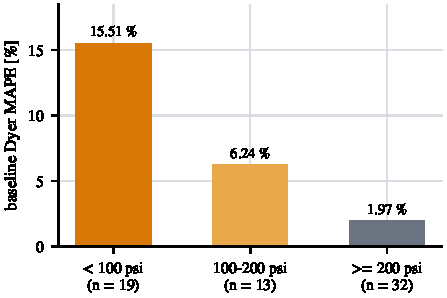
\includegraphics[width=.62\textwidth]{fig_baseline_bands.pdf}
\caption{Baseline Dyer MAPE in the three supercharge bands of Table~\ref{tab:base}. The same model, with the same Cd, goes from 2\,\% to 15.5\,\% as the tank loses its subcooling margin.}
\label{fig:bands}
\end{figure}

A second motivation appeared while testing the correction. For a saturated inlet $\kappa=1$, so Dyer's prediction there is $(\mdot_{SPI}+\mdot_{HEM})/2$, whereas the project's model for a fluid arriving already partially vaporised is pure HEM, which at $x_{inlet}\to0$ is the flow just across the flashing threshold. Hence
\begin{equation}
\frac{\mdot_{Dyer}}{\mdot_{HEM}}\Big|_{\text{threshold}}=\frac{1+\mdot_{SPI}/\mdot_{HEM}}{2},
\label{eq:jump}
\end{equation}
about 1.16 at the Waxman conditions but about 1.75 in the project's Example~3 ($\mdot_{SPI}/\mdot_{HEM}\approx2.5$). The statement that HEM ``gives half the Dyer flow'' therefore holds only when $\mdot_{SPI}\gg\mdot_{HEM}$. The discontinuity makes the damped fixed-point solver alternate between the two branches, and fail to converge, in a narrow band of tank pressures.

The main results of this version are:
\begin{enumerate}[label=(\roman*)]
\item \emph{The correction generalises.} Out of sample, MAPE $6.88\to1.36\,\%$, maximum error $33.5\to11.6\,\%$, bias $+6.7\to-0.4\,\%$ (Table~\ref{tab:pooled}); the held-out 41~psi curve goes from $17.8$ to $4.1\,\%$ (Fig.~\ref{fig:folds}).
\item \emph{The gate is not identified; one parameter suffices.} The optimum lies at the edge of the data ($S_0\approx400$~psi); $\kappa'\simeq\kappa S/S_0$ gives $1.17\,\%$ against $1.30\,\%$ for two parameters (Table~\ref{tab:forms}).
\item \emph{It is not a Cd shift}, and it improves a second geometry that never entered a fit when evaluated with its measured Cd ($4.47\to1.26\,\%$, Table~\ref{tab:partA2}).
\item \emph{It removes the threshold discontinuity.} Dyer joins HEM as $S\to0$; the solver failure band of Example~3 (6/25 and 5/25 pressures) vanishes (Table~\ref{tab:scan}).
\item \emph{Limits.} One rig, one injector, 280--283~K: the correction is not adopted as the default (Section~\ref{sec:status}).
\end{enumerate}

%====================================================================== II
\section{Why $\kappa$ Degrades at Low Supercharge: Primary-Source Support}\label{sec:source}
Equation~\eqref{eq:dyer} is derived, and its interpretation discussed, by Vargas Ni\~no and Razavi~\cite{nino2019}, already the source of this project's original four-point validation subset (their Table~4); their Eq.~(4) is identical to Eq.~\eqref{eq:dyer}. Discussing the approach to saturation, the authors state:
\begin{quote}\small
``At saturated conditions the NHNE model loses its physical interpretation as the value of $\kappa$ is unity and the resulting mass flux\ldots\ is simply an equal averaging of the SPI and HEM models.''
\end{quote}
This is a statement from the model's own literature that $\kappa$ degenerates to a supercharge-independent value ($\kappa=1$) exactly in the regime where Table~\ref{tab:base} shows the largest error. The same paper goes further: for a different model (their ``Omega'' formulation, an equation-of-state approach distinct from Dyer/NHNE) it introduces a supercharge threshold $\eta_{st}$ that classifies each operating point as high or low supercharged and, in the low branch, applies
\begin{equation}
G=\frac{P_{sat}}{P_i}\,G_{sat}+\Bigl(1-\frac{P_{sat}}{P_i}\Bigr)G_{low},
\label{eq:omega}
\end{equation}
justified by ``the sharp edge effect increasing the tendency for cavitation, which is more prevalent in the predictions of the saturated mass flux equation.'' This is direct precedent, in a source already cited, for a regime-gated correction at low supercharge, applied here to Dyer's $\kappa$ because re-deriving the Omega formulation is a substantially larger undertaking. Table~\ref{tab:source} summarises what each source is used for.

\begin{table}[!htbp]
\centering\small
\caption{Literature used as support, and what each item supports.}
\label{tab:source}
\begin{tabular}{p{3.9cm}p{6.2cm}p{4.4cm}}\toprule
Source & Statement & Used for\\\midrule
Vargas Ni\~no \& Razavi (2019), discussion of Eq.~(4) & $\kappa=1$ at saturation: NHNE becomes an equal average of SPI and HEM & Diagnosis: $\kappa$ degenerates where the error is largest\\
Vargas Ni\~no \& Razavi (2019), Omega model & Supercharge threshold $\eta_{st}$; low-supercharge blend, Eq.~\eqref{eq:omega} & Precedent for a regime-gated correction\\
Vargas Ni\~no \& Razavi (2019), discharge coefficients & Cd about 0.73 (high supercharge) versus about 0.85 (low) & Cd and supercharge regime are not separable\\
Waxman et al.\ (2013) & Finite rate of interphase heat and mass transfer against residence time & Physical meaning of $\kappa$\\\bottomrule
\end{tabular}
\end{table}

%====================================================================== III
\section{Proposed Correction}\label{sec:correction}
The working hypothesis of version~1 is a gated modification of $\kappa$,
\begin{equation}
\kappa'=\begin{cases}\kappa, & S\geq S_{ref},\\[2pt] \kappa\,(S/S_{ref})^{\beta}, & S<S_{ref},\end{cases}
\label{eq:gate}
\end{equation}
with two free parameters, the exponent $\beta\geq0$ and the threshold $S_{ref}$. A power law is used, rather than an exponential or another two-parameter attenuating form, because it is the simplest form satisfying $\kappa'(S{=}0)=0$ together with independent control of curvature via $\beta$. The limit $S\to0$ corresponds to the tank sitting exactly on the saturation curve, where the non-equilibrium picture underlying $\kappa$ (a finite bubble-growth delay relative to residence time) is least applicable and the flow is expected to approach equilibrium (the HEM limit, $\kappa\to0$) fastest. Four properties follow directly from Eq.~\eqref{eq:gate} (Table~\ref{tab:props}).

\subsection{Exact recovery}
For any $S\geq S_{ref}$, $\kappa'=\kappa$ exactly, regardless of $\beta$; likewise $\beta=0$ gives $\kappa'=\kappa$ everywhere. The correction is inert unless both $S<S_{ref}$ and $\beta>0$.

\subsection{Continuity at the threshold}
Both one-sided limits at $S_{ref}$ equal $\kappa$, so $\kappa'$ and the Dyer flow computed from it are continuous ($C^0$) across the gate for any $\beta\geq0$. The continuity is $C^0$ only: the slope changes from $\kappa\beta/S_{ref}$ immediately below $S_{ref}$ to that of $\kappa$ above it (a kink). A Jacobian-based solver could in principle be more sensitive there; none has been observed with the project's damped fixed-point iteration.

\subsection{Monotonicity}
Below $S_{ref}$, $\kappa'$ is the product of two increasing functions of $S$ (at fixed $P_{down}$ and $T_{up}$ the original $\kappa$ itself increases with $S$, Eq.~\eqref{eq:identity}), and the Dyer blend is monotonic in $\kappa$ for fixed SPI and HEM endpoints (Section~\ref{sec:sens}). No spurious extrema are introduced inside $(0,S_{ref})$.

\subsection{A dimensionless identity and the HEM limit}\label{sec:identity}
Since $P_{up}-P_{down}=S+(P_{sat}-P_{down})$,
\begin{equation}
\kappa^2=1+\frac{S}{D},\qquad D\equiv P_{sat}(T_{up})-P_{down},
\label{eq:identity}
\end{equation}
so $\kappa^2-1=S/D$ is a dimensionless supercharge, and any multiplier $f(S)$ with $f(0)=0$ gives $\kappa'\to0$ and Eq.~\eqref{eq:blend}$\to\mdot_{HEM}$ as $S\to0$. That is exactly the flow of the two-phase-inlet branch at $x_{inlet}\to0$: the discontinuity of Eq.~\eqref{eq:jump} disappears by construction.

\begin{table}[!htbp]
\centering\small
\caption{Properties of the gated form, Eq.~\eqref{eq:gate}.}
\label{tab:props}
\begin{tabular}{p{2.8cm}p{6.0cm}p{5.9cm}}\toprule
Property & Statement & Consequence\\\midrule
Exact recovery & $\kappa'=\kappa$ for $S\geq S_{ref}$ or $\beta=0$ & Previously published predictions above $S_{ref}$ are untouched\\
Continuity & $C^0$ at $S_{ref}$; slope kink & No jump in $\mdot$ at the gate\\
Monotonicity & $\kappa'$ increasing in $S$ below $S_{ref}$ & No spurious extrema\\
HEM limit & $\kappa'\to0$ as $S\to0$ ($\beta>0$) & Dyer $\to$ HEM at the flashing threshold\\\bottomrule
\end{tabular}
\end{table}

%====================================================================== IV
\section{Version 1: Grid Search on the Digitised Dataset (In-Sample)}\label{sec:v1}
\subsection{Grid search over the two parameters}
Cd is calibrated once, pooled over the single-phase windows of all nine injector-3 curves ($\mathrm{Cd}=0.781$), independently of $\beta$ and $S_{ref}$. A grid search over $\beta\in[0,3]$ and $S_{ref}\in[50,300]$~psi against the 64 two-phase points yielded two representative operating points (Table~\ref{tab:grid}). The unrestricted variant reduces the global MAPE by a factor 3.7 at the cost of 2.02 percentage points in the four-point Part~A subset.

\begin{table}[!htbp]
\centering\small
\caption{Version~1: two representative points of the $(\beta,S_{ref})$ grid search. All figures are \emph{in-sample} (fitted and measured on the same 64 points); see Section~\ref{sec:loocv} for the out-of-sample result. ``Protects Part A'': $S_{ref}$ below Part~A's own supercharge ($\approx$95~psi), so $\kappa'=\kappa$ exactly for those four points.}
\label{tab:grid}
\begin{tabular}{lrrrrc}\toprule
Variant & $S_{ref}$ [psi] & $\beta$ & Global MAPE & Part A MAPE & Protects Part A?\\\midrule
Baseline (no correction) & --- & 0 & 6.86\,\% & 2.75\,\% & ---\\
Conservative & 80 & 2.5 & 4.63\,\% & 2.75\,\% & yes\\
Unrestricted & 300 & 1.0 & 1.86\,\% & 4.77\,\% & no\\\bottomrule
\end{tabular}
\end{table}

\subsection{A structural fact about Part A's supercharge}
Part~A's four points (Table~4 of Ref.~\cite{nino2019}; injector~2; $\Delta P=8$--14~bar) have a tank supercharge of only $\approx$95~psi ($\approx$6.55~bar): inside the low-supercharge regime the correction targets, not safely above it. Any $S_{ref}\geq95$~psi therefore necessarily perturbs Part~A, and the ``protects Part~A'' variants are those whose $S_{ref}$ is too low to reach the 100--200~psi band, where the baseline error is also elevated (Table~\ref{tab:base}). No choice of $S_{ref}$ corrects that band while leaving Part~A untouched: a structural property of the dataset, not a shortcoming of the grid search.

%====================================================================== V
\section{Out-of-Sample Test of the Hypothesis}\label{sec:loocv}
The headline of version~1 (1.86\,\%) has an obvious weakness: two parameters were fitted on the same points on which the error is reported. This section tests the hypothesis out of sample.

\subsection{Protocol}
Leave-one-curve-out cross-validation over the nine supercharge curves (Table~\ref{tab:protocol}). The grid was fixed before any out-of-sample result was seen. Two fitting variants are run: \emph{free}, and \emph{protected} ($S_{ref}\leq94.7$~psi, leaving Part~A untouched by construction). A second analysis (``mode~B'') fits Cd jointly with the correction on the training points, to test whether the correction is a disguised Cd shift. Table~\ref{tab:base} uses the Cd pooled over all curves; in the LOOCV the Cd of each fold excludes the held-out curve (0.779--0.782), so baseline figures differ slightly (6.88\,\% against 6.85\,\%).

\begin{table}[!htbp]
\centering\small
\caption{Leave-one-curve-out protocol, repeated for each of the nine supercharge curves $k$.}
\label{tab:protocol}
\begin{tabular}{p{.9cm}p{8.6cm}p{5.1cm}}\toprule
Step & Action & Excluded from it\\\midrule
1 & Calibrate Cd on the single-phase windows ($30~\text{psi}\leq\Delta P\leq S$) of the other eight curves & Curve $k$ (not even through Cd)\\
2 & Fit the correction on the two-phase points of those eight curves, minimising their MAPE on a fixed grid: $\beta\in[0,3]$ (step 0.1), $S_{ref}\in[20,400]$~psi (step 5) & Curve $k$; Part~A\\
3 & Predict the two-phase points of curve $k$ with the fitted parameters and the fold Cd & ---\\
$+$ & Evaluate Part~A (injector~2) with the parameters fitted on all injector-3 data & Never enters any fit\\\bottomrule
\end{tabular}
\end{table}

\subsection{Result: the correction generalises}
Figure~\ref{fig:folds} shows each held-out curve and Table~\ref{tab:folds} the numbers behind it; Table~\ref{tab:pooled} gives the pooled result.

\begin{figure}[!htbp]
\centering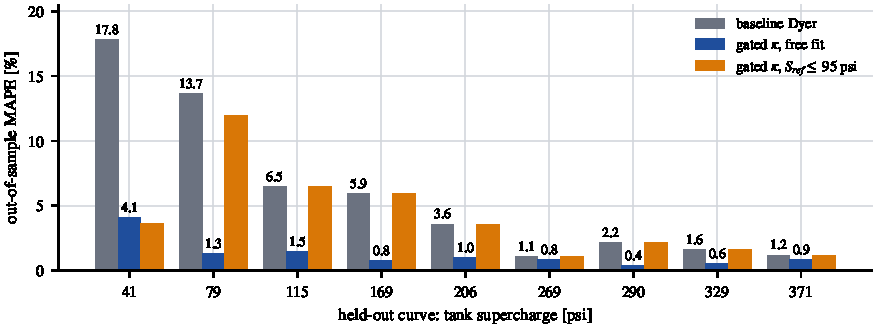
\includegraphics[width=.95\textwidth]{fig_loocv_folds.pdf}
\caption{Out-of-sample error per held-out curve. Each group of bars is one supercharge level; the prediction for that curve comes from a model fitted on the other eight. Grey: baseline Dyer. Blue: gated $\kappa$ with free parameters. Orange: gated $\kappa$ restricted to $S_{ref}\leq95$~psi. The free fit is never worse than the baseline; the protected variant helps only below about 100~psi.}
\label{fig:folds}
\end{figure}

\begin{table}[!htbp]
\centering\small
\caption{Per-fold out-of-sample MAPE [\%]; parameters chosen on the other eight curves.}
\label{tab:folds}
\begin{tabular}{rrrrcr}\toprule
$S$ [psi] & $n$ & Base & Free & $\beta/S_{ref}$ & Prot.\\\midrule
41 & 9 & 17.80 & 4.07 & 1.1/385 & 3.65\\
79 & 10 & 13.67 & 1.31 & 0.9/400 & 11.93\\
115 & 7 & 6.50 & 1.48 & 0.9/400 & 6.50\\
169 & 6 & 5.93 & 0.75 & 1.0/395 & 5.93\\
206 & 6 & 3.58 & 1.00 & 1.0/395 & 3.58\\
269 & 5 & 1.08 & 0.84 & 1.0/400 & 1.08\\
290 & 8 & 2.16 & 0.39 & 1.0/400 & 2.16\\
329 & 7 & 1.60 & 0.55 & 1.0/400 & 1.60\\
371 & 6 & 1.19 & 0.87 & 0.9/400 & 1.19\\\bottomrule
\end{tabular}
\end{table}

\begin{table}[!htbp]
\centering\small
\caption{Pooled out-of-sample results over the 64 two-phase points. The in-sample free fit gives 1.11\,\% ($\beta=1.0$, $S_{ref}=400$~psi).}
\label{tab:pooled}
\begin{tabular}{lrrr}\toprule
 & Mean & MAPE & max $|$err$|$\\\midrule
Baseline Dyer & $+6.72\,\%$ & 6.88\,\% & 33.5\,\%\\
Gated, free fit & $-0.35\,\%$ & \textbf{1.36\,\%} & 11.6\,\%\\
Gated, $S_{ref}\leq95$ psi & $+3.50\,\%$ & 4.62\,\% & 25.4\,\%\\\bottomrule
\end{tabular}
\end{table}

By band (Fig.~\ref{fig:lbands}), out of sample: below 100~psi $15.6\to2.6\,\%$; 100--200~psi $6.2\to1.1\,\%$; above 200~psi $1.95\to0.70\,\%$. The 41~psi curve, the only one close to saturation and hence a genuine extrapolation towards the threshold, goes from $17.8$ to $4.1\,\%$ (maximum error $33.5\to11.6\,\%$). The fitted parameters are stable across the nine folds ($\beta=0.9$--1.1, $S_{ref}=385$--400~psi).

\begin{figure}[!htbp]
\centering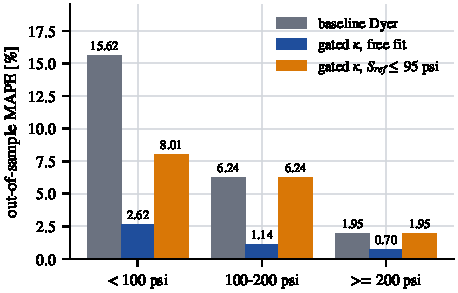
\includegraphics[width=.66\textwidth]{fig_loocv_bands.pdf}
\caption{Out-of-sample MAPE by supercharge band. The free fit lowers the error in every band, most of all where the baseline fails; the protected variant changes only the lowest band.}
\label{fig:lbands}
\end{figure}

\subsection{Revision of the hypothesis: a rescaling, not a gate}
The optimum $S_{ref}=400$~psi lies at the edge of the grid and above the highest supercharge measured (371~psi): all 64 points lie on the corrected branch, so the data identify an approximately linear rescaling $\kappa'\simeq\kappa S/S_0$, not a gate. (The 1.86\,\% of version~1 was likewise a grid-edge optimum, at the then upper limit of 300~psi.) The protected variant fails (4.62\,\%) because it acts only below 100~psi, whereas Dyer's over-prediction extends well beyond: the conflict with Part~A noted in Section~\ref{sec:v1} is a Cd issue, not a gate issue (Section~\ref{sec:cd}).

To find the simplest form that does the job, seven multipliers $f$ of $\kappa$ were compared (Table~\ref{tab:formdef}, Fig.~\ref{fig:shapes}), with $S_{ref}$ allowed up to 3000~psi.

\begin{table}[!htbp]
\centering\small
\caption{Candidate forms. $f$ multiplies $\kappa$; $D=P_{sat}-P_{down}$, so $\kappa^2-1=S/D$ (Eq.~\eqref{eq:identity}).}
\label{tab:formdef}
\begin{tabular}{llcccc}\toprule
Form & $f$ & Parameters & $f\to0$ as $S\to0$ & Bounded by 1 & Dimensionless\\\midrule
F0 baseline Dyer & $1$ & 0 & no & yes & ---\\
F1 gated power & Eq.~\eqref{eq:gate} & 2 & yes & yes & no\\
F2 linear & $S/S_0$ & 1 & yes & no (cap needed) & no\\
F4 & $\sqrt{\kappa^2-1}/\kappa$ & 0 & yes & yes & yes\\
F5 & $(\kappa^2-1)/\kappa$ & 0 & yes & no & yes\\
F6 soft gate & $S/(S+S_1)$ & 1 & yes & yes & no\\
F7 soft gate, exponent & $(S/(S+S_1))^{\beta}$ & 2 & yes & yes & no\\\bottomrule
\end{tabular}
\end{table}

\begin{figure}[!htbp]
\centering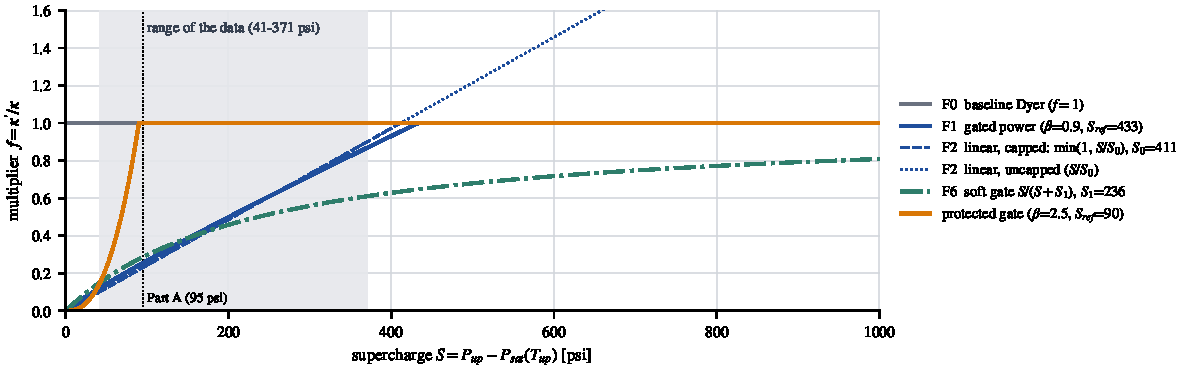
\includegraphics[width=.95\textwidth]{fig_factor_shapes.pdf}
\caption{Effect of each candidate on $\kappa$. The vertical axis is the multiplier $f=\kappa'/\kappa$ (1 = no correction); fitted parameters as in Table~\ref{tab:stab}. The shaded band is the range of supercharge covered by the data (41--371~psi); outside it every curve is an extrapolation. Inside it the fitted forms F1, F2 and F6 are close to one another, which is why the data cannot tell them apart; they differ widely above 371~psi. The orange curve is the protected gate, already equal to 1 above 90~psi.}
\label{fig:shapes}
\end{figure}

\begin{figure}[!htbp]
\centering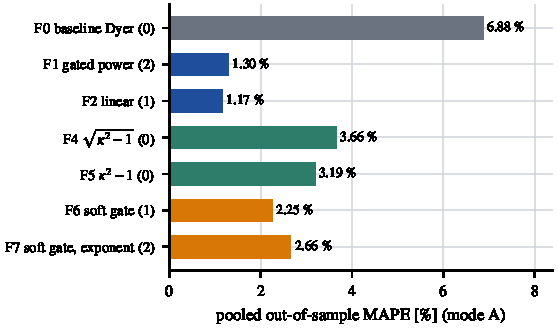
\includegraphics[width=.66\textwidth]{fig_forms.pdf}
\caption{Pooled out-of-sample MAPE of the seven forms (mode~A, Cd from the single-phase windows); the number in brackets is the count of fitted parameters. Grey: baseline; blue: hard or linear gates; orange: soft gates; green: parameter-free dimensionless forms.}
\label{fig:forms}
\end{figure}

\begin{table}[!htbp]
\centering\small
\caption{Out-of-sample comparison (MAPE [\%]). Mode~A: Cd from the single-phase windows. Mode~B: Cd fitted jointly. Part~A uses the parameters fitted on all injector-3 data, with the generic and the measured Cd.}
\label{tab:forms}
\begin{tabular}{lcrrrrr}\toprule
Form & Parameters & Pooled A & Pooled B & 41 psi (A) & Part A, Cd 0.65 & Part A, Cd 0.681\\\midrule
F0 baseline Dyer & 0 & 6.88 & 6.08 & 17.80 & 2.75 & 4.47\\
F1 gated power & 2 & 1.30 & 1.28 & 4.08 & 5.51 & 1.21\\
\textbf{F2 linear} & \textbf{1} & \textbf{1.17} & 1.19 & 3.42 & 5.83 & 1.34\\
F4 & 0 & 3.66 & 3.65 & 7.72 & 2.56 & 3.31\\
F5 & 0 & 3.19 & 2.10 & 2.98 & 1.79 & 3.94\\
F6 soft gate & 1 & 2.25 & 2.07 & 2.17 & 5.11 & 1.15\\
F7 soft gate, exponent & 2 & 2.66 & 2.14 & 4.69 & 5.00 & 1.13\\\bottomrule
\end{tabular}
\end{table}

A single parameter does as well as two. The two parameter-free forms F4 and F5, dimensionless by Eq.~\eqref{eq:identity}, cost 3--4\,\% MAPE. Seven forms were compared on the same data and the best was not selected inside the cross-validation, so 1.17\,\% is slightly optimistic; a planning figure is 1.2--1.5\,\%.

\begin{table}[!htbp]
\centering\small
\caption{Stability of the fitted parameters over the nine folds (mode~A), and behaviour of the multiplier $f=\kappa'/\kappa$ outside the data (in-sample fit); the data end at 371~psi.}
\label{tab:stab}
\begin{tabular}{llcrrrrrr}\toprule
 & & & \multicolumn{6}{c}{$f$ at $S$ [psi]}\\\cmidrule(l){4-9}
Form & Parameter, range over folds & In-sample & 41 & 100 & 200 & 371 & 600 & 1000\\\midrule
F1 & $\beta$ 0.9--1.1; $S_{ref}$ 386--433 & 0.9 / 433 & 0.12 & 0.27 & 0.50 & 0.87 & 1.00 & 1.00\\
F2 & $S_0$ 380--411 & 411 & 0.10 & 0.24 & 0.49 & 0.90 & 1.46 & 2.43\\
F6 & $S_1$ 172--262 & 236 & 0.15 & 0.30 & 0.46 & 0.61 & 0.72 & 0.81\\
F7 & $\beta$ 1.5--3.0; $S_1$ 36--128 & 2.0 / 79 & 0.12 & 0.31 & 0.51 & 0.68 & 0.78 & 0.86\\\bottomrule
\end{tabular}
\end{table}

\subsection{It is not a disguised Cd shift}
If Dyer's over-prediction were a mis-calibrated Cd, fitting Cd jointly (mode~B) would remove most of it. It does not (Table~\ref{tab:cdb}): the baseline improves only from 6.88\,\% to 6.08\,\% (Cd $=0.755$ against 0.781), whereas every corrected form selects Cd $=0.76$--0.79, essentially the single-phase value. The correction acts on $\kappa$, not on Cd.

\begin{table}[!htbp]
\centering\small
\caption{Cd selected by the joint fit (mode~B). The pooled single-phase value is 0.781.}
\label{tab:cdb}
\begin{tabular}{lcc}\toprule
Form & Cd over folds & Cd in-sample\\\midrule
F0 baseline Dyer & 0.750--0.760 & 0.755\\
F1 gated power & 0.785--0.790 & 0.785\\
F2 linear & 0.785 & 0.785\\
F4 & 0.770--0.775 & 0.775\\
F5 & 0.760--0.765 & 0.760\\
F6 soft gate & 0.790 & 0.790\\
F7 soft gate, exp. & 0.785--0.790 & 0.790\\\bottomrule
\end{tabular}
\end{table}

\subsection{Part A: a second geometry}
Across the nine fold parameter sets the Part~A MAPE ranges 5.27--6.06\,\% (Cd 0.65) and 1.17--1.58\,\% (Cd 0.681) (Table~\ref{tab:partA2}). With the measured Cd the correction lowers the error from 4.47\,\% to 1.2--1.3\,\% on a geometry it never saw; with the generic Cd the model under-predicts (mean $-5.7\,\%$), as expected if the true Cd of injector~2 is higher than 0.65. This supports reading the original 2.76\,\% as a favourable cancellation between Dyer's over-prediction and an under-estimated Cd (an inference: four points, one supercharge level).

\subsection{The flashing threshold and the coupled solver}
Figure~\ref{fig:limit} (numbers in Table~\ref{tab:limit}) checks the argument of Section~\ref{sec:identity}: as the supercharge goes to zero the corrected prediction tends to HEM, while the uncorrected Dyer stays at the factor of Eq.~\eqref{eq:jump}.

\begin{figure}[!htbp]
\centering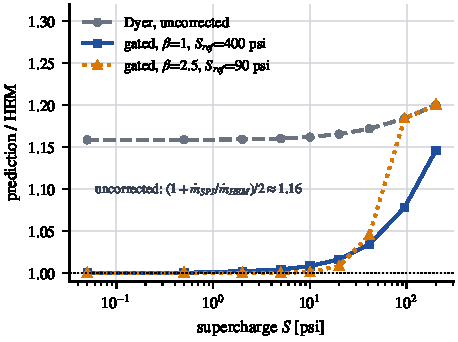
\includegraphics[width=.66\textwidth]{fig_limit.pdf}
\caption{Prediction divided by the HEM flow as the supercharge $S$ goes to zero ($T=280$~K, $P_{down}=30$~bar). A ratio of 1 means no discontinuity with the two-phase-inlet branch. The uncorrected Dyer (dashed) stays at $(1+\mdot_{SPI}/\mdot_{HEM})/2\approx1.16$; the corrected variants reach 1.000 below 1~psi.}
\label{fig:limit}
\end{figure}

\begin{table}[!htbp]
\centering\small
\caption{Prediction/HEM against supercharge (values plotted in Fig.~\ref{fig:limit}).}
\label{tab:limit}
\begin{tabular}{rccc}\toprule
$S$ [psi] & Dyer & $\beta{=}1$, 400 & $\beta{=}2.5$, 90\\\midrule
0.05 & 1.158 & 1.000 & 1.000\\
0.5 & 1.158 & 1.000 & 1.000\\
2 & 1.159 & 1.002 & 1.000\\
5 & 1.160 & 1.004 & 1.000\\
10 & 1.162 & 1.008 & 1.001\\
20 & 1.165 & 1.016 & 1.008\\
41 & 1.171 & 1.034 & 1.045\\
95 & 1.184 & 1.078 & 1.184\\
200 & 1.200 & 1.146 & 1.200\\\bottomrule
\end{tabular}
\end{table}

Inside the coupled solver (optional argument \code{kappa_correction}), the tank pressure was scanned from 52 to 58~bar for the two line geometries of Example~3 (Fig.~\ref{fig:scan}, Tables~\ref{tab:scan} and~\ref{tab:ex3}).

\begin{figure}[!htbp]
\centering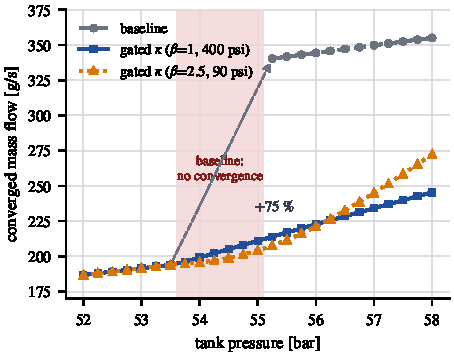
\includegraphics[width=.70\textwidth]{fig_scan.pdf}
\caption{Converged oxidiser mass flow against tank pressure for the original Example~3 geometry (needle valve, 8~mm line, 22~$^\circ$C, 18~bar chamber). The baseline (dashed) stops converging between 53.75 and 55.00~bar (shaded) and, where it converges again, has jumped by $+75\,\%$ (193.9 to 340.3~g/s) because the model switched from the HEM two-phase-inlet branch to Dyer. The corrected model converges everywhere and varies smoothly.}
\label{fig:scan}
\end{figure}

\begin{table}[!htbp]
\centering\small
\caption{Tank-pressure scan, 52--58~bar in 0.25~bar steps (25 pressures per geometry). ``Largest jump'': largest relative change of the converged flow between adjacent pressures; for the baseline it is the change across the non-converging band.}
\label{tab:scan}
\begin{tabular}{llcccc}\toprule
Geometry & Variant & Non-converging & Largest jump & Flow at 58 bar [g/s]\\\midrule
\multirow{3}{*}{needle valve, 8 mm} & baseline & 6/25 (53.75--55.00 bar) & $\approx+75\,\%$ (band) & 355.1\\
 & $\beta=1$, 400 psi & 0/25 & 1.5\,\% & 245.4\\
 & $\beta=2.5$, 90 psi & 0/25 & 2.7\,\% & 272.4\\\midrule
\multirow{3}{*}{ball valve, 8 mm} & baseline & 5/25 (53.50--54.50 bar) & $\approx+76\,\%$ (band) & 358.6\\
 & $\beta=1$, 400 psi & 0/25 & 1.6\,\% & 248.8\\
 & $\beta=2.5$, 90 psi & 0/25 & 2.9\,\% & 283.9\\\bottomrule
\end{tabular}
\end{table}

\begin{table}[!htbp]
\centering\small
\caption{Example~3 recomputed [g/s]. The Henry--Fauske ceiling no longer binds with the correction (ceilings 259--279~g/s against corrected flows of 195--247~g/s).}
\label{tab:ex3}
\begin{tabular}{lrrr}\toprule
Step & Base & $\beta{=}1$, 400 & $\beta{=}2.5$, 90\\\midrule
0: 53.5 bar, needle & 193.9 & 193.9 & 193.9\\
1: ball valve & no conv. & 195.4 & 194.6\\
2: 56 bar & 347.7 & 225.6 & 226.8\\
3: 12~mm line & 356.2 & 233.7 & 246.9\\\bottomrule
\end{tabular}
\end{table}

The gain from raising the tank pressure from 53.5 to 56~bar is $+79\,\%$ in the baseline and $+16\,\%$ with the correction. At 58~bar the two corrected variants differ by about 10\,\% (245 and 272~g/s): the model uncertainty at this operating point. These figures extrapolate from the Waxman data (280--283~K, one injector) to 295~K and another geometry; they are not validated there.

%====================================================================== VI
\section{Interaction With Discharge-Coefficient Calibration}\label{sec:cd}
Part~A's four points were originally evaluated, here and in Ref.~\cite{nino2019}, with Cd $=0.65$, a generic value. Waxman's Fig.~15~\cite{waxman2013} reports a directly measured Cd $=0.681$ for this injector-2 geometry. Tables~\ref{tab:partA1} and~\ref{tab:partA2} isolate the effect of this substitution, with and without the correction.

\begin{table}[!htbp]
\centering\small
\caption{Version~1: Part~A MAPE under the four combinations of Cd and correction ($\beta=1$, $S_{ref}=300$~psi, the in-sample parameters of Table~\ref{tab:grid}).}
\label{tab:partA1}
\begin{tabular}{lrr}\toprule
 & No correction & Corrected\\\midrule
Cd $=0.65$ (generic) & 2.75\,\% & 4.77\,\%\\
Cd $=0.681$ (measured) & 4.47\,\% & 1.14\,\%\\\bottomrule
\end{tabular}
\end{table}

\begin{table}[!htbp]
\centering\small
\caption{Version~2: the same comparison with the cross-validated parameters ($\beta=1$, $S_{ref}=400$~psi, fitted on injector~3 only); range over the nine fold parameter sets.}
\label{tab:partA2}
\begin{tabular}{lrrr}\toprule
 & No corr. & Corrected & Folds\\\midrule
Cd $=0.65$ & 2.75\,\% & 5.74\,\% & 5.27--6.06\\
Cd $=0.681$ & 4.47\,\% & \textbf{1.26\,\%} & 1.17--1.58\\\bottomrule
\end{tabular}
\end{table}

With the measured Cd the correction does not degrade Part~A: it improves it substantially, below even the originally published baseline. Neither factor in isolation explains the improvement: the measured Cd alone worsens the uncorrected baseline ($2.75\to4.47\,\%$), and the correction alone (with the generic Cd) also worsens it. Only the combination improves it. This is an interaction, not one effect ``explaining away'' the other; version~2 adds that it is not an artefact of fitting Cd and the correction on the same injector (Table~\ref{tab:cdb}).

\subsection{Independent support}
Vargas Ni\~no and Razavi~\cite{nino2019} report that the appropriate Cd differs by supercharge regime (about 0.73 for high supercharge, from a cavitation-number correlation, against about 0.85 suggested for low supercharge) and that their regime-corrected Omega model, Eq.~\eqref{eq:omega}, already absorbs part of this difference, making a third, dedicated Cd unnecessary. This is independent, primary-source support for the qualitative finding of Table~\ref{tab:partA2}.

%====================================================================== VII
\section{A First-Order Sensitivity Argument}\label{sec:sens}
The interaction can be given an order-of-magnitude account by linearising the Dyer prediction in its two calibration inputs, Cd and $\kappa'$. Writing the blend explicitly,
\begin{equation}
\mdot_{Dyer}=\frac{C_dA\sqrt{2\Delta P}}{\kappa'+1}\Bigl(\kappa'\sqrt{\rho_l}+\sqrt{\rho_{HEM}}\Bigr),
\label{eq:explicit}
\end{equation}
differentiation gives, exactly,
\begin{equation}
\frac{\partial\ln\mdot_{Dyer}}{\partial\kappa'}=\frac{\sqrt{\rho_l}-\sqrt{\rho_{HEM}}}{(\kappa'+1)\bigl(\kappa'\sqrt{\rho_l}+\sqrt{\rho_{HEM}}\bigr)}>0,
\label{eq:deriv}
\end{equation}
positive whenever $\rho_l>\rho_{HEM}$ (always once vapour is present): a larger $\kappa'$ shifts the blend towards SPI, which predicts more flow than HEM. Decreasing $\kappa'$, the direction the correction imposes at low supercharge, therefore lowers the prediction. Since $\partial\ln\mdot_{Dyer}/\partial\ln C_d=1$, a first-order expansion around a nominal point gives
\begin{equation}
\frac{d\mdot_{Dyer}}{\mdot_{Dyer}}=\frac{dC_d}{C_d}+C_\varphi\frac{d\kappa'}{\kappa'_0},\quad
C_\varphi\equiv\kappa'_0\,\frac{\partial\ln\mdot_{Dyer}}{\partial\kappa'}\Big|_0>0.
\label{eq:taylor}
\end{equation}
The quantity reported is the relative error $E\equiv(\mdot_{Dyer}-\mdot_{exp})/\mdot_{exp}$; near a calibration point where the model already tracks the data ($|E_0|\ll1$), $dE\approx d\mdot_{Dyer}/\mdot_{Dyer}$, so
\begin{equation}
\Delta E\approx\frac{\Delta C_d}{C_{d,0}}+C_\varphi\frac{\Delta\kappa'}{\kappa'_0}.
\label{eq:dE}
\end{equation}
An error sourced from Cd and one sourced from $\kappa'$ therefore enter the total additively at first order: a poorly chosen Cd and a correction calibrated against data evaluated with that same Cd partly compensate one another, as in Tables~\ref{tab:partA1} and~\ref{tab:partA2}. This is a local, linearised statement, adequate for the direction and approximate scale of the interaction; it is not a derivation of $\beta$ or $S_{ref}$, which would require, e.g., a bubble-growth or nucleation-delay model (Section~\ref{sec:future}).

%====================================================================== VIII
\section{What This Work Does Not Establish}\label{sec:not}
Table~\ref{tab:claims} gives the status of each claim; the points below expand on those that are not established.

\begin{table}[!htbp]
\centering\small
\caption{Status of each claim.}
\label{tab:claims}
\begin{tabular}{p{4.5cm}p{6.8cm}p{3.5cm}}\toprule
Claim & Evidence & Status\\\midrule
Dyer over-predicts at low supercharge & 64 points, injector 3 (one rig) & Established (one geometry)\\
The correction lowers the error out of sample on injector 3 & LOOCV, $6.88\to1.36\,\%$; 41 psi curve held out & Established within the data range\\
One parameter suffices & Table~\ref{tab:forms}: F2 1.17\,\% against F1 1.30\,\% & Supported\\
It is not a Cd shift & Mode~B, Table~\ref{tab:cdb} & Supported (injector 3)\\
It transfers to another geometry & Part~A: $4.47\to1.26\,\%$ with measured Cd; 4 points, one supercharge & Weak evidence\\
It transfers to other temperatures & None; Example~3 is at 295~K & Not established\\
Behaviour above 371~psi & None (Table~\ref{tab:stab}) & Not established\\
Dyer $\to$ HEM continuous at the threshold & Analytic (Eq.~\eqref{eq:identity}), Table~\ref{tab:limit}, solver scan & Established (a property of the form)\\
The HEM branch is right near the threshold & No data below 41~psi & Not established\\
Physical mechanism (sharp-edge cavitation) & Analogy with Ref.~\cite{nino2019} & Hypothesis\\\bottomrule
\end{tabular}
\end{table}

\begin{itemize}
\item \textbf{$S_0$ has no physical scaling.} It is expressed in psi; whether it scales with $P_{sat}$, with the subcooling $\Delta T_{sub}$, or stays fixed cannot be told from data at 280--283~K. The dimensionless forms F4/F5 avoid the ambiguity but fit worse (3--4\,\%).
\item \textbf{Supercharge above 371~psi.} F2 grows without bound ($f=2.4$ at 1000~psi); the defensible form is $\kappa\min(1,S/S_0)$, identical on the data and equal to the original Dyer above $S_0$, but its cap is untested. The bounded soft gate F6 saturates at $\kappa$ by construction.
\item \textbf{Model selection.} Seven forms were compared on the same 64 points; the best is not selected inside the cross-validation.
\item \textbf{The HEM branch itself.} The correction removes the artificial jump at the threshold, not a possible error in the HEM two-phase-inlet branch, which has no experimental validation. The data reach only $S\geq41$~psi; below that, the HEM limit follows from the functional form, not from an observation.
\item \textbf{Mechanism.} The mechanism proposed by Vargas Ni\~no and Razavi (sharp orifice-edge geometry increasing cavitation tendency) is geometry-specific; whether it transfers to a correction of $\kappa$ has not been checked against CFD or a nucleation model, only against aggregate mass-flow data.
\item \textbf{Choking.} No claim is made about two-phase choking in the metastable mixture. The connection to the project's choking diagnostics (Henry--Fauske~\cite{henry1971}, HEM critical flow) has not been tested; in Example~3 the corrected flows fall below the Henry--Fauske ceiling.
\item \textbf{Parameters are empirical.} $\beta$, $S_{ref}$ and $S_0$ are fitted to this project's own digitised dataset, not derived from a primary source the way $\kappa$ itself or the Henry--Fauske ceiling are; they should not be treated as universal constants.
\end{itemize}

%====================================================================== IX
\section{Conclusions and Status}\label{sec:status}
A supercharge-dependent reduction of Dyer's $\kappa$ lowers the out-of-sample error of the two-phase predictions from 6.9\,\% to 1.4\,\% on the available data, behaves consistently on a second injector geometry when evaluated with its measured Cd, and makes the Dyer and HEM branches continuous at the flashing threshold. The data support a one-parameter linear rescaling rather than the gate originally hypothesised. The correction is nevertheless fitted to one injector at 280--283~K and is exploratory: it is not the model's default.

In the software it is available as an optional argument \code{kappa_correction} of \code{evaluate_full_system()} and \code{design_injector_area()} (default \code{None}: every result unchanged; tests in \code{tests/test_kappa_correction_option.py}). In the Dyer regime the interactive tool shows a warning beside the unchanged Dyer result, with the flow the correction would give (Sizing mode) or the orifice area it would require (Design mode), using $\beta=1$ and $S_{ref}=400$~psi; the same note is added to the PDF export, and is reduced to a one-line caption when the correction changes the result by less than 2\,\%.

Before the correction is promoted to a default the following are required: (a)~independent data (another injector geometry, or another temperature) on which the parameters fitted here are tested without refitting; (b)~a decision between the capped linear form, a bounded soft gate and a dimensionless form; (c)~validation of the HEM two-phase-inlet branch, on which the corrected model relies near the threshold.

%====================================================================== X
\section{Future Work}\label{sec:future}
\begin{enumerate}
\item \textbf{Independent geometry and temperature.} Acquire or digitise low-supercharge two-phase data for another injector, and for temperatures away from 280--283~K, to test whether the parameters fitted on injector~3 generalise and whether $S_0$ scales with $P_{sat}$ or $\Delta T_{sub}$. Cold-flow measurements at fixed, large $\Delta P$ over a range of supercharge would be the most direct test.
\item \textbf{First-principles threshold.} Relate $S_{ref}$ (or $S_0$) to a time-scale ratio (residence time in the orifice against a bubble-growth or nucleation-delay time) instead of fitting it, as the Henry--Fauske ceiling is derived rather than fitted.
\item \textbf{Decoupled Cd calibration.} Recalibrate Cd per injector geometry before any new parameter search (Section~\ref{sec:cd}).
\item \textbf{HEM branch.} Validate the two-phase-inlet model, or replace the Dyer$\to$HEM switch by a single continuous model.
\end{enumerate}

%====================================================================== XI
\section{Reproducibility}\label{sec:repro}
All results are produced by scripts in the repository (Table~\ref{tab:repro}); each writes a text output in \code{validation/kappa_correction/}. The scripts reuse the loaders and Cd calibration of \code{validation/waxman_2013_validation.py}. The correction itself is \code{dyer_mass_flow_corrected()} in \code{src/model/injector_two_phase.py}. The written account is in \code{validation/waxman_2013_results.md}, Sections~10 and~11, and the tracking in \code{docs/future_work.md}, Priority~1.

\begin{table}[!htbp]
\centering\small
\caption{Where each result comes from.}
\label{tab:repro}
\begin{tabular}{p{6.4cm}p{6.7cm}p{1.8cm}}\toprule
Script & Produces & Sections\\\midrule
\code{validation/explore_supercharge_correction.py} & Version~1 grid search, Part~A with both Cd (Tables~\ref{tab:grid}, \ref{tab:partA1}) & \ref{sec:v1}, \ref{sec:cd}\\
\code{validation/kappa_correction/loocv_kappa_correction.py} & Per-fold and pooled results, Part~A, limit check (Tables~\ref{tab:folds}, \ref{tab:pooled}, \ref{tab:partA2}, \ref{tab:limit}) & \ref{sec:loocv}\\
\code{validation/kappa_correction/loocv_functional_forms.py} & Candidate forms, modes A/B, stability (Tables~\ref{tab:forms}, \ref{tab:stab}, \ref{tab:cdb}) & \ref{sec:loocv}\\
\code{validation/kappa_correction/scan_threshold_continuity.py} & Tank-pressure scan and Example~3 (Tables~\ref{tab:scan}, \ref{tab:ex3}) & \ref{sec:loocv}\\
\code{docs/reports/figures/make_figures.py} & All figures of this report & ---\\\bottomrule
\end{tabular}
\end{table}

\begin{thebibliography}{9}\footnotesize
\bibitem{dyer2007} Dyer, J., Doran, E., Dunn, Z., Lohner, K., Zilliac, G., and Cantwell, B., ``Modeling Feed System Flow Physics for Self-Pressurizing Propellants,'' AIAA Paper 2007-5702, 2007.
\bibitem{solomon2011} Solomon, B. J., ``Engineering Model to Calculate Mass Flow Rate of a Two-Phase Saturated Fluid through an Injector Orifice,'' M.Sc. Thesis, Utah State University, 2011.
\bibitem{waxman2013} Waxman, B. S., Zimmerman, J. E., Cantwell, B., and Zilliac, G., ``Mass Flow Rate and Isolation Characteristics of Injectors for Use with Self-Pressurizing Oxidizers in Hybrid Rockets,'' AIAA Paper 2013-3636, 2013.
\bibitem{nino2019} Vargas Ni\~no, E., and Razavi, M. R. H., ``Design of Two-Phase Injectors Using Analytical and Numerical Methods with Application to Hybrid Rockets,'' AIAA Propulsion and Energy 2019 Forum, AIAA Paper 2019-4154, 2019.
\bibitem{henry1971} Henry, R. E., and Fauske, H. K., ``The Two-Phase Critical Flow of One-Component Mixtures in Nozzles, Orifices, and Short Tubes,'' \emph{ASME Journal of Heat Transfer}, Vol.~93, No.~2, 1971, pp.~179--187.
\end{thebibliography}
\end{document}
